\section{Модальный регулятор}
Рассмотрим систему: 
\begin{equation}
    \dot{x} = Ax + Bu
\end{equation}
где 
\begin{equation}
    \begin{array}{cc}
        A = \begin{bmatrix}
            8 & 1 & 11 \\ 
            4 & 0 & 4 \\
            -4 & -3 & -7
        \end{bmatrix}, &
        B = \begin{bmatrix}
            -1 \\ -3 \\ 3
        \end{bmatrix}
    \end{array}
\end{equation}

\subsection{Управляемость собственных чисел}

Для определения управляемости собственных чисел рассмотрим вещественную Жорданову форму системы: 
\begin{equation}
    \dot{\hat{x}} = P^{-1}AP\hat{x} + P^{-1}Bu
\end{equation}
Где $P$ -- матрица собственных векторов матрицы $A$, а $\hat{x} = P^{-1}x$.
\begin{equation}
    A_j = \begin{bmatrix}
        -3  & 0  & 0 \\ 
        0  & 2  & -2 \\ 
        0  & 2  & 2 \\ 
    \end{bmatrix}\quad
    P = \begin{bmatrix}
        -1  & -2.12  & 0.71 \\ 
        0  & -1.41  & 0 \\ 
        1  & 1.41  & 0 \\ 
    \end{bmatrix}\quad 
    B_j = \begin{bmatrix}
        0 \\ 
        2.12 \\ 
        4.95 \\ 
    \end{bmatrix}
\end{equation}

Таким образом, последнее собственное число $\lambda_3 = -3$ не является управляемым. Соответственно, система не является полностью управляемой. 
Но, так как данное собственное число располагается в левой полуплоскости, то есть является устойчивым, то система является стабилизируемой. 

\subsection{Модальный регулятор}
Замкнем систему обратной связью с модальным регулятором $u = -Kx$. Тогда уравнение состояния системы примет вид:
\begin{equation}
    \dot{x} = Ax - BKx = (A - BK)x 
\end{equation}
Моделировать данную данную систему будем с помощью среды моделирования Simulink. Схема моделирования представлена на рисунке \ref{fig:scheme1}. 
\begin{figure}[ht!]
    \centering
    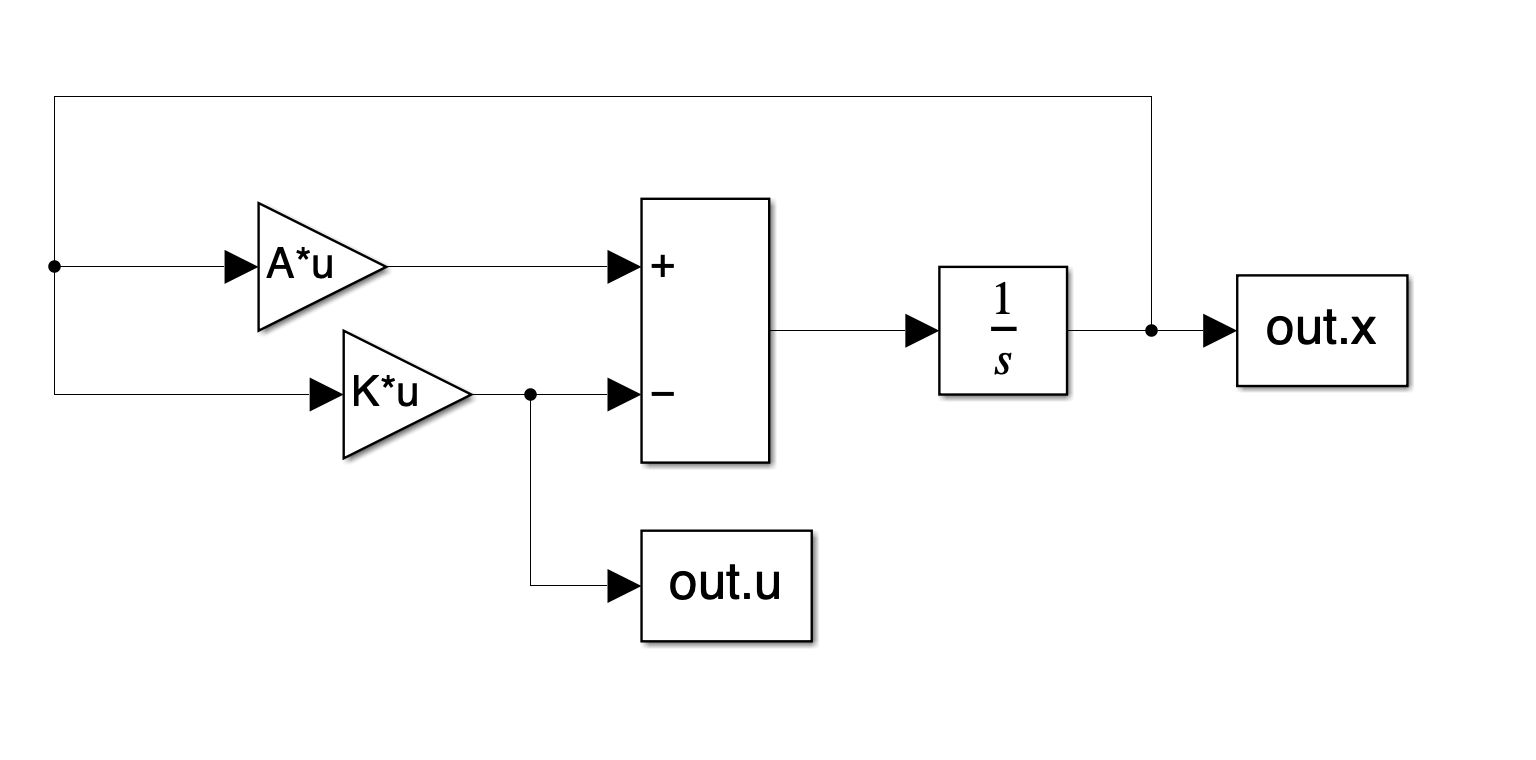
\includegraphics[width=\textwidth]{media/scheme1.png}
    \caption{Схема моделирования системы с модальным регулятором}
    \label{fig:scheme1}
\end{figure}

\subsubsection{Подбор спектра модального регулятора}
Рассмотрим следующие варианты спектра модального регулятора: 
\begin{enumerate}
    \item $\sigma_1 = \left\{ -1, -1, -1 \right\}$
    \item $\sigma_2 = \left\{ -3, -3, -3 \right\}$
    \item $\sigma_3 = \left\{ -1, -10, -100 \right\}$
    \item $\sigma_4 = \left\{ -3, -30, -300 \right\}$
    \item $\sigma_5 = \left\{ -1, -1\pm3i \right\}$
    \item $\sigma_6 = \left\{ -3, -3\pm9i \right\}$
\end{enumerate}

Так как одно из собственных чисел матрицы $A$ не является управляемым, то есть ни одно входное воздействие, а значит и ни один регулятор 
не может управлять данным собственным числом, то спектр замкнутой системы не может не содержать данное собственное число. 
Следовательно, спектры $\sigma_1$, $\sigma_3$, $\sigma_5$ не являются допустимыми.

Для того, чтобы проверить, может ли спектр системы, замкнутой модальным регулятором, быть равен заданному спектру $\sigma_i$, 
нужно проверить, подобна ли матрица $A + BK$ матрице $\Gamma_i$ с заданным спектром $\sigma_i$.
Матрицу $\Gamma_i$ можно называть эталонной системой.

Для упрощения задачи подбора регулятора можно \textit{сократить} систему, убрав из нее неуправляемые собственные числа. 
Для этого уберем строку и столбец в диагональной форме, соответствующие неуправляемому собственному числу $\lambda_1 = -3$:
\begin{equation}
    \dot{\hat{x}}' =
     \begin{bmatrix}
        2  & -2 \\ 
        2  & 2 \\
    \end{bmatrix} \hat{x}' + 
    \begin{bmatrix}
        2.12 \\ 
        4.95 \\ 
    \end{bmatrix}u
\end{equation}

Найдем вектор управления в Жордановой форме $K_j$ с помощью метода Аккермана (с помощью одноименной функции в Matlab) для эталонной системы $\Gamma_i$: 
\begin{equation}
    K_j = \begin{bmatrix}
        -1.06  & 2.47 \\ 
    \end{bmatrix}
\end{equation}

Теперь вернемся к полной системе, поставив в векторе $K$ нулевое значение для неуправляемого собственного числа: 
\begin{equation}
    K_j = \begin{bmatrix}
        0  & -1.06  & 2.47 \\ 
    \end{bmatrix}
\end{equation}
Вернемся к исходному базису:
\begin{equation}
    K = K_jP^{-1} = \begin{bmatrix}
        3.48 & -1 & 3.48
    \end{bmatrix}
\end{equation}
В итоге получим систему: 
\begin{eqnarray}
    \dot{x} = Ax - BKx = (A - BK)x = \begin{bmatrix}
        11.48 & 0 & 14.48 \\
    14.44 & -3 & 14.44 \\
    -14.44 & 0 & -17.44
    \end{bmatrix} x
\end{eqnarray}
Можно проверить, найдя ее собственные числа. Спектр системы: $\sigma_2 = \left\{ -3, -3, -3 \right\}$.

\subsubsection{Моделирование}
Проведем моделирование системы с модальным регулятором, спектр которого равен $\sigma_2$ и начальными условиями $x(0) = \begin{bmatrix} 1 & 1 & 1 \end{bmatrix}^T$.
Результаты моделирования представлены на рисунке \ref{fig:task1_u_2} и \ref{fig:task1_x_2}.
\begin{figure}[ht!]
    \centering
    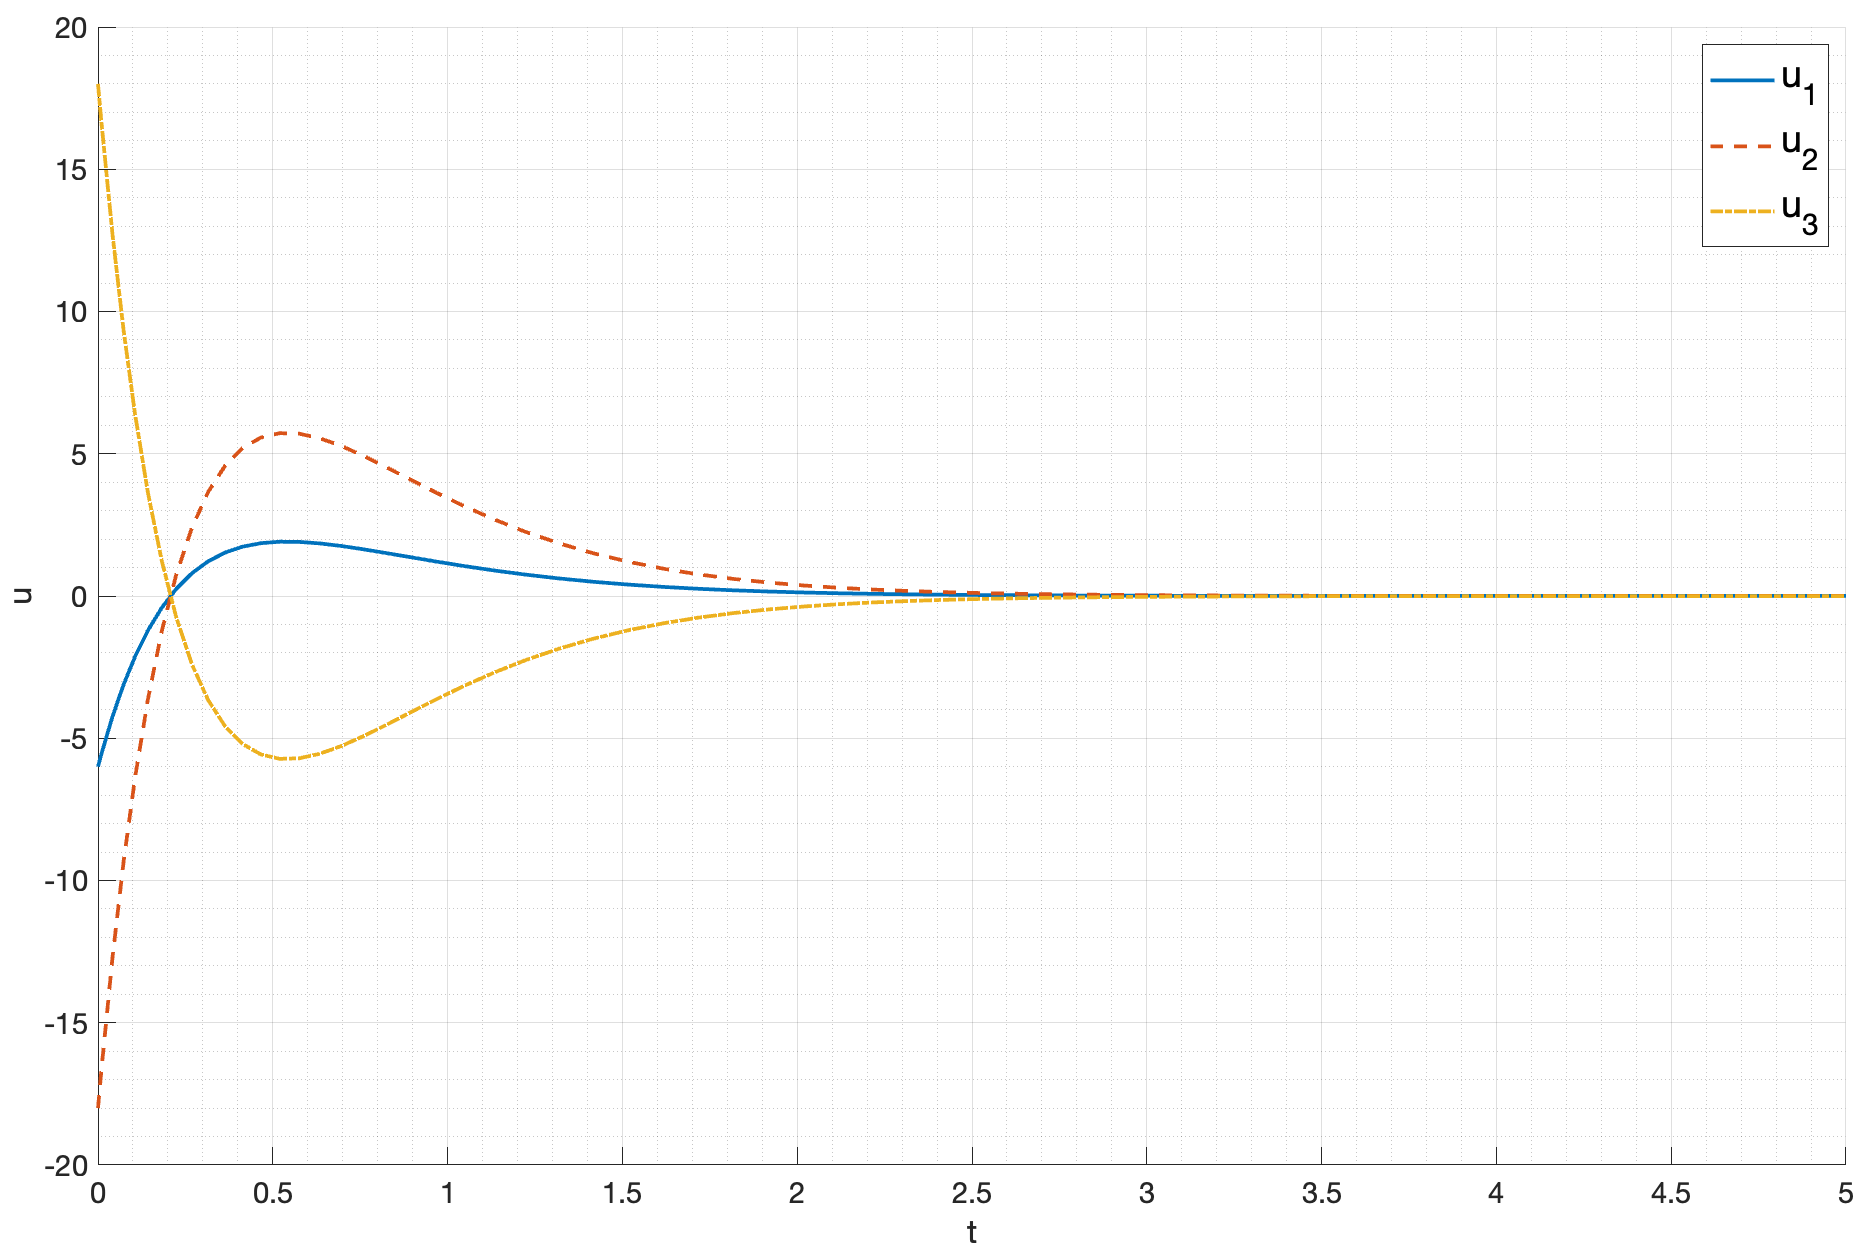
\includegraphics[width=\textwidth]{media/plots/task1_u_2.png}
    \caption{Управление системы со спектром $\sigma_2$}
    \label{fig:task1_u_2}
\end{figure}
\begin{figure}
    \centering
    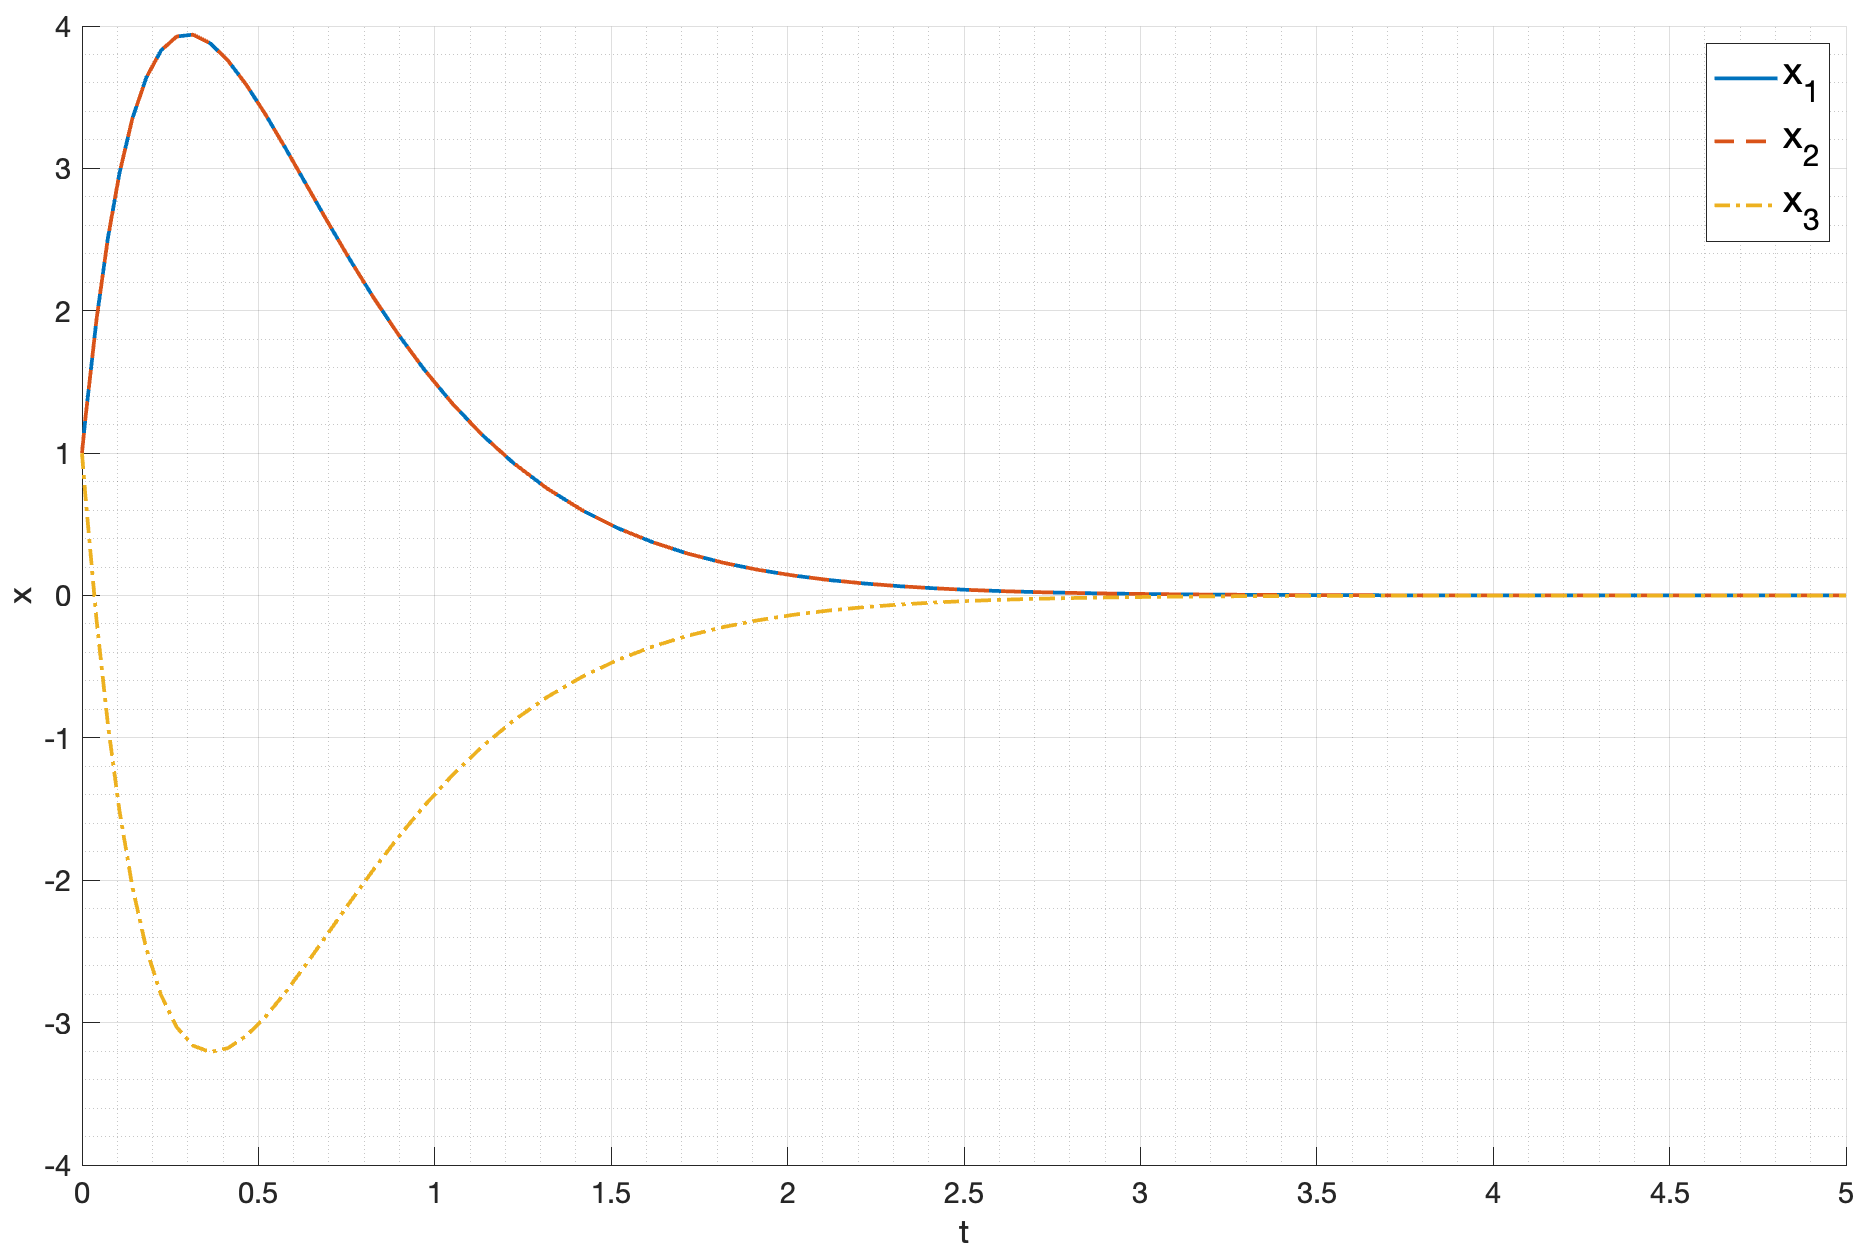
\includegraphics[width=\textwidth]{media/plots/task1_x_2.png}
    \caption{Состояние системы со спектром $\sigma_2$}
    \label{fig:task1_x_2}
\end{figure}

Аналогично найдем регулятор для спектра $\sigma_4$:
\begin{equation}
    K = \begin{bmatrix}
        580.28  & 275.52  & 580.28 \\ 
    \end{bmatrix}
\end{equation}
\begin{equation}
    \dot{x} = Ax - BKx = (A - BK)x = \begin{bmatrix}
        588.28  & 276.52  & 591.28 \\ 
        1744.83  & 826.55  & 1744.83 \\ 
        -1744.83  & -829.55  & -1747.83 \\ 
    \end{bmatrix}x
\end{equation}
Спектр системы: $\sigma_4 = \left\{ -3, -30, -300 \right\}$.
Результаты моделирования представлены на рисунках \ref{fig:task1_u_4} и \ref{fig:task1_x_4}.
\begin{figure}[ht!]
    \centering
    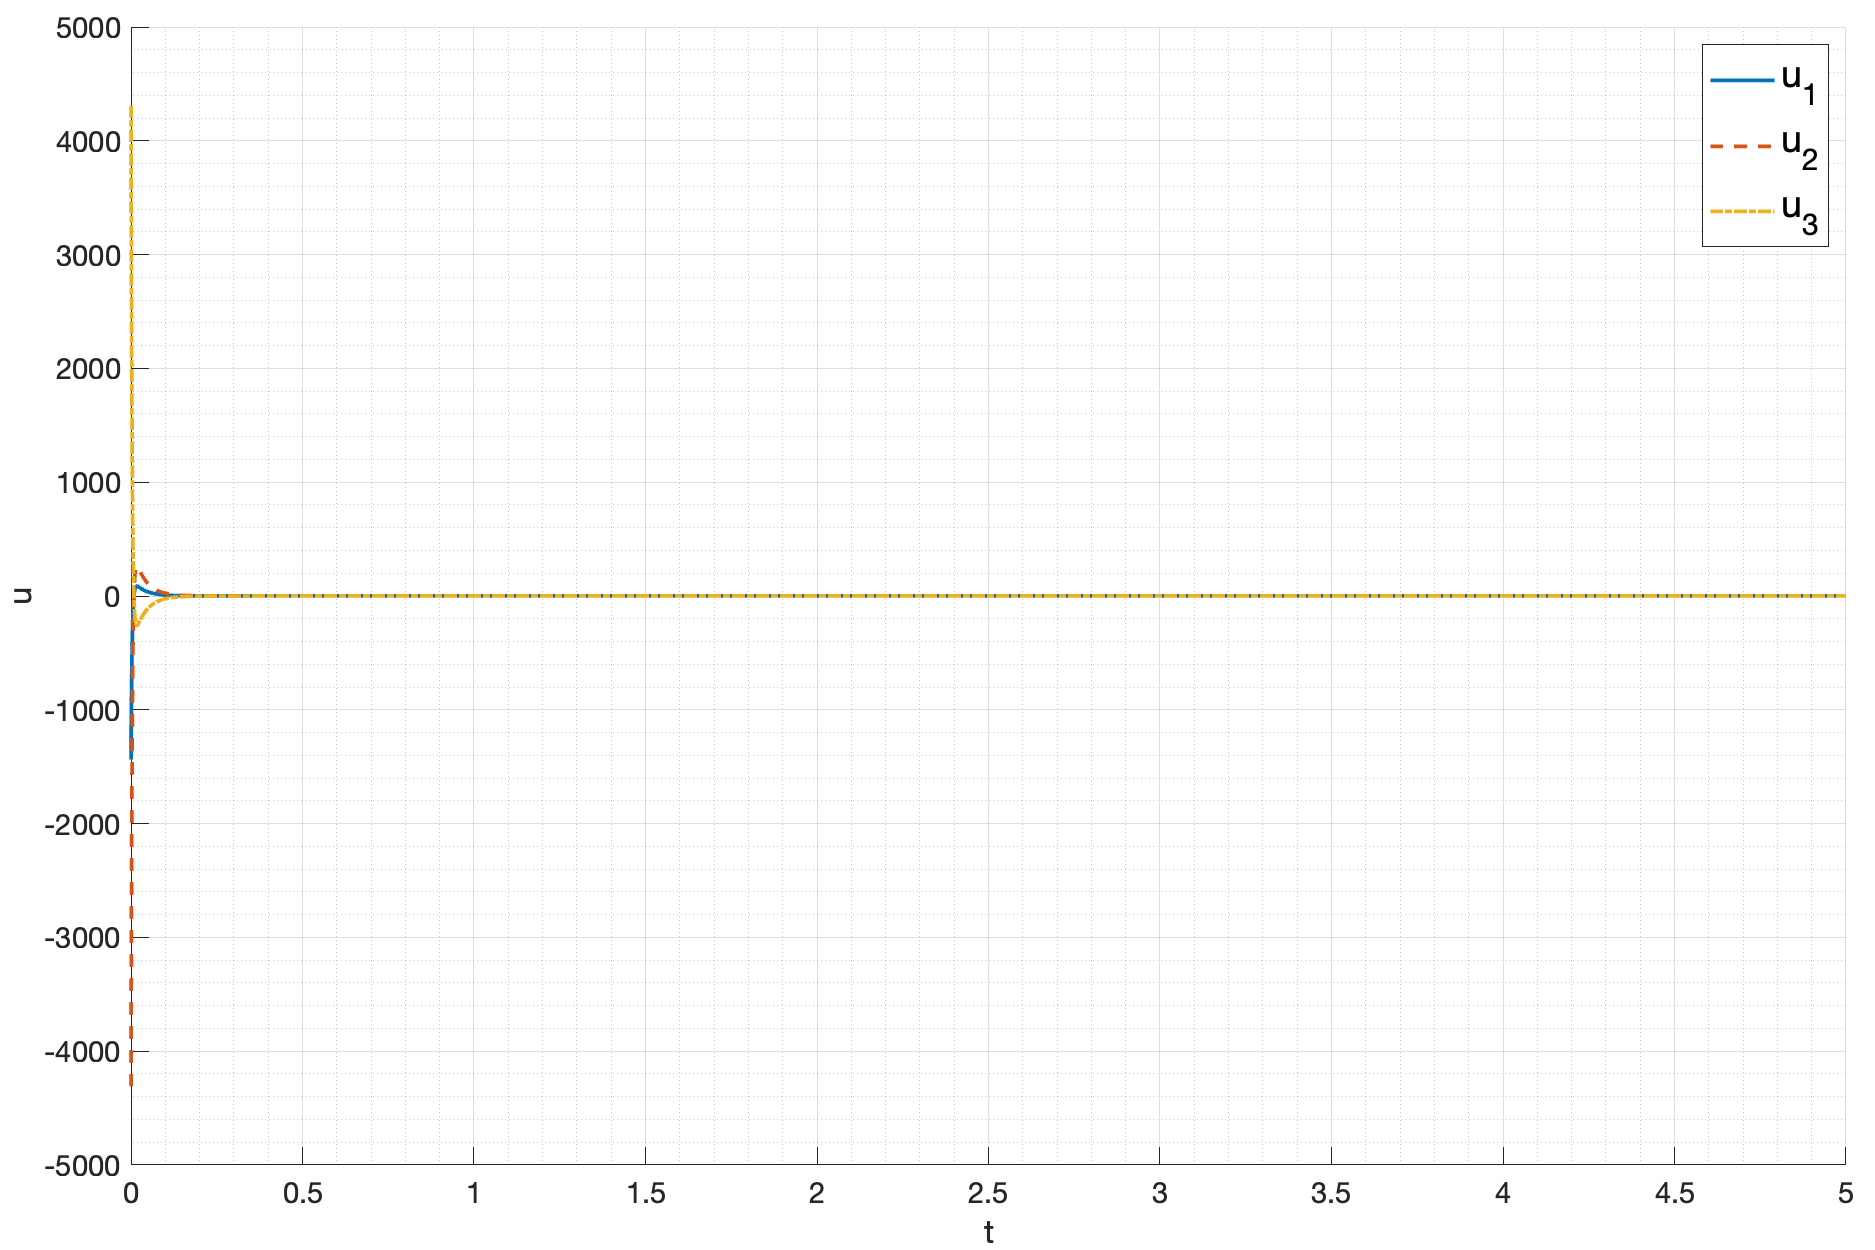
\includegraphics[width=\textwidth]{media/plots/task1_u_4.png}
    \caption{Управление системы со спектром $\sigma_4$}
    \label{fig:task1_u_4}
\end{figure}
\begin{figure}
    \centering
    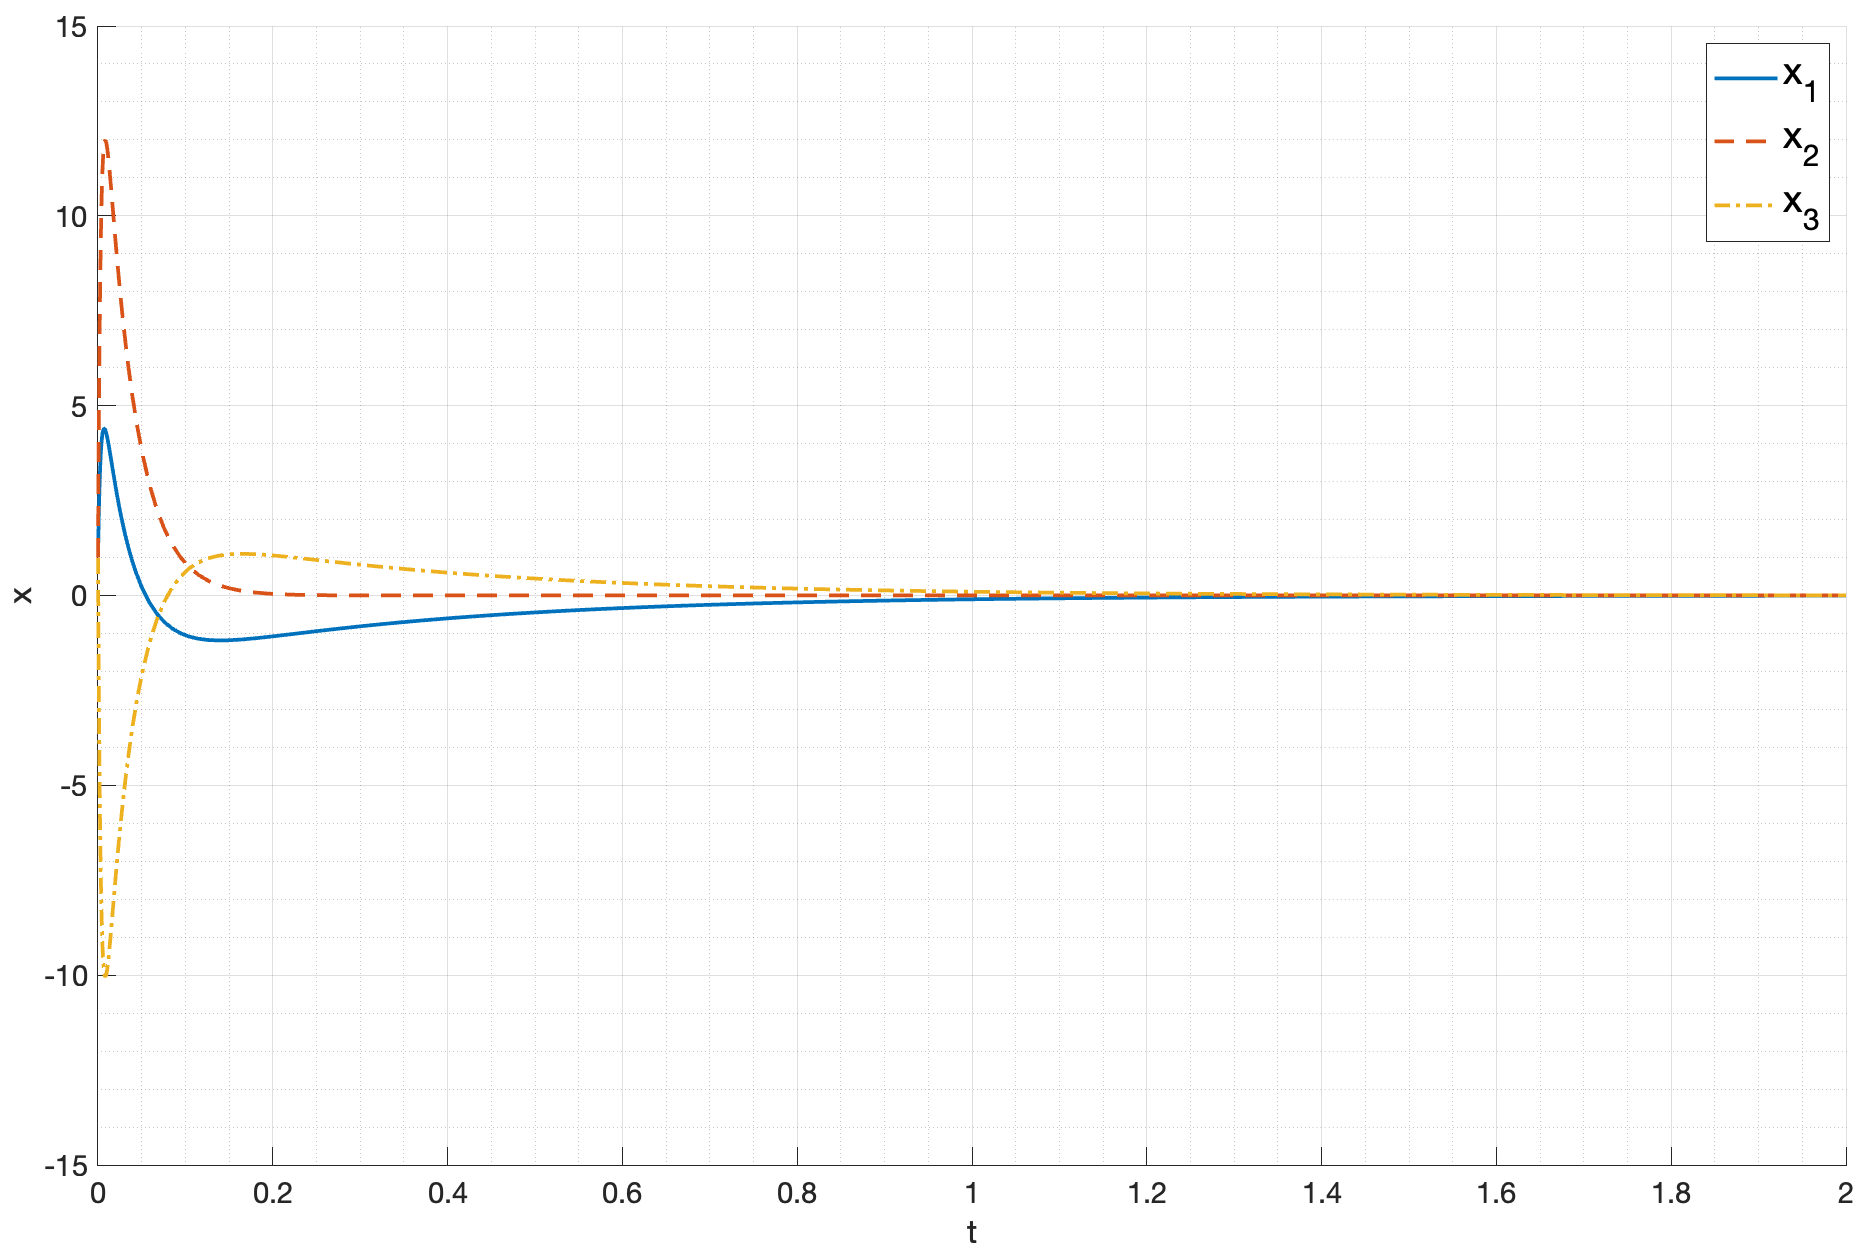
\includegraphics[width=\textwidth]{media/plots/task1_x_4.png}
    \caption{Состояние системы со спектром $\sigma_4$}
    \label{fig:task1_x_4}
\end{figure}

И для спектра $\sigma_6$:
\begin{equation}
    K = \begin{bmatrix}
        7.69  & 1.79  & 7.69 \\ 
    \end{bmatrix}
\end{equation}
\begin{equation}
    \dot{x} = Ax - BKx = (A - BK)x = \begin{bmatrix}
        15.69  & 2.79  & 18.69 \\ 
        27.07  & 5.38  & 27.07 \\ 
        -27.07  & -8.38  & -30.07 \\ 
    \end{bmatrix}x
\end{equation}
Спектр системы: $\sigma_6 = \left\{ -3, -3\pm9i \right\}$.
Результаты моделирования представлены на рисунках \ref{fig:task1_u_6} и \ref{fig:task1_x_6}.
\begin{figure}[ht!]
    \centering
    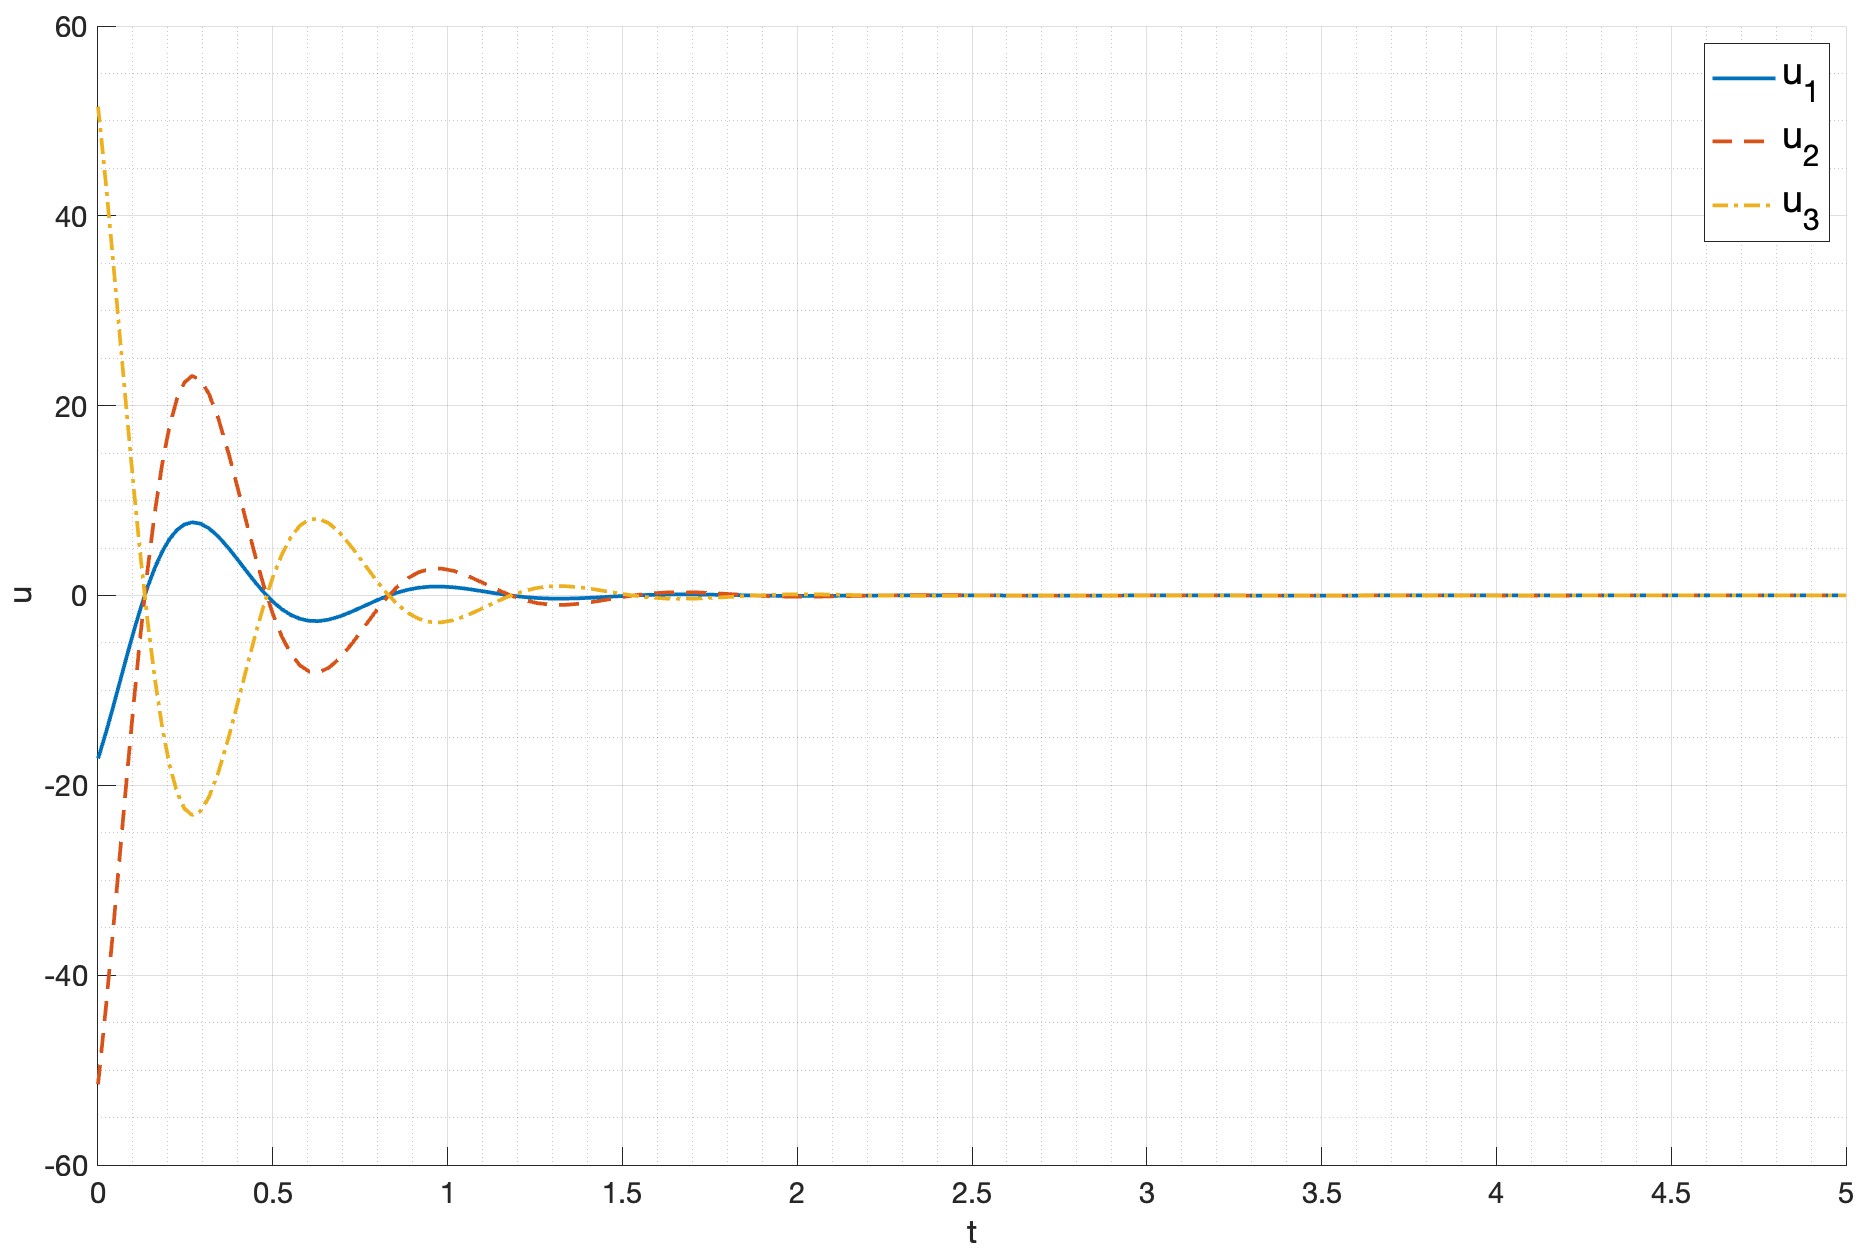
\includegraphics[width=\textwidth]{media/plots/task1_u_6.png}
    \caption{Управление системы со спектром $\sigma_6$}
    \label{fig:task1_u_6}
\end{figure}
\begin{figure}
    \centering
    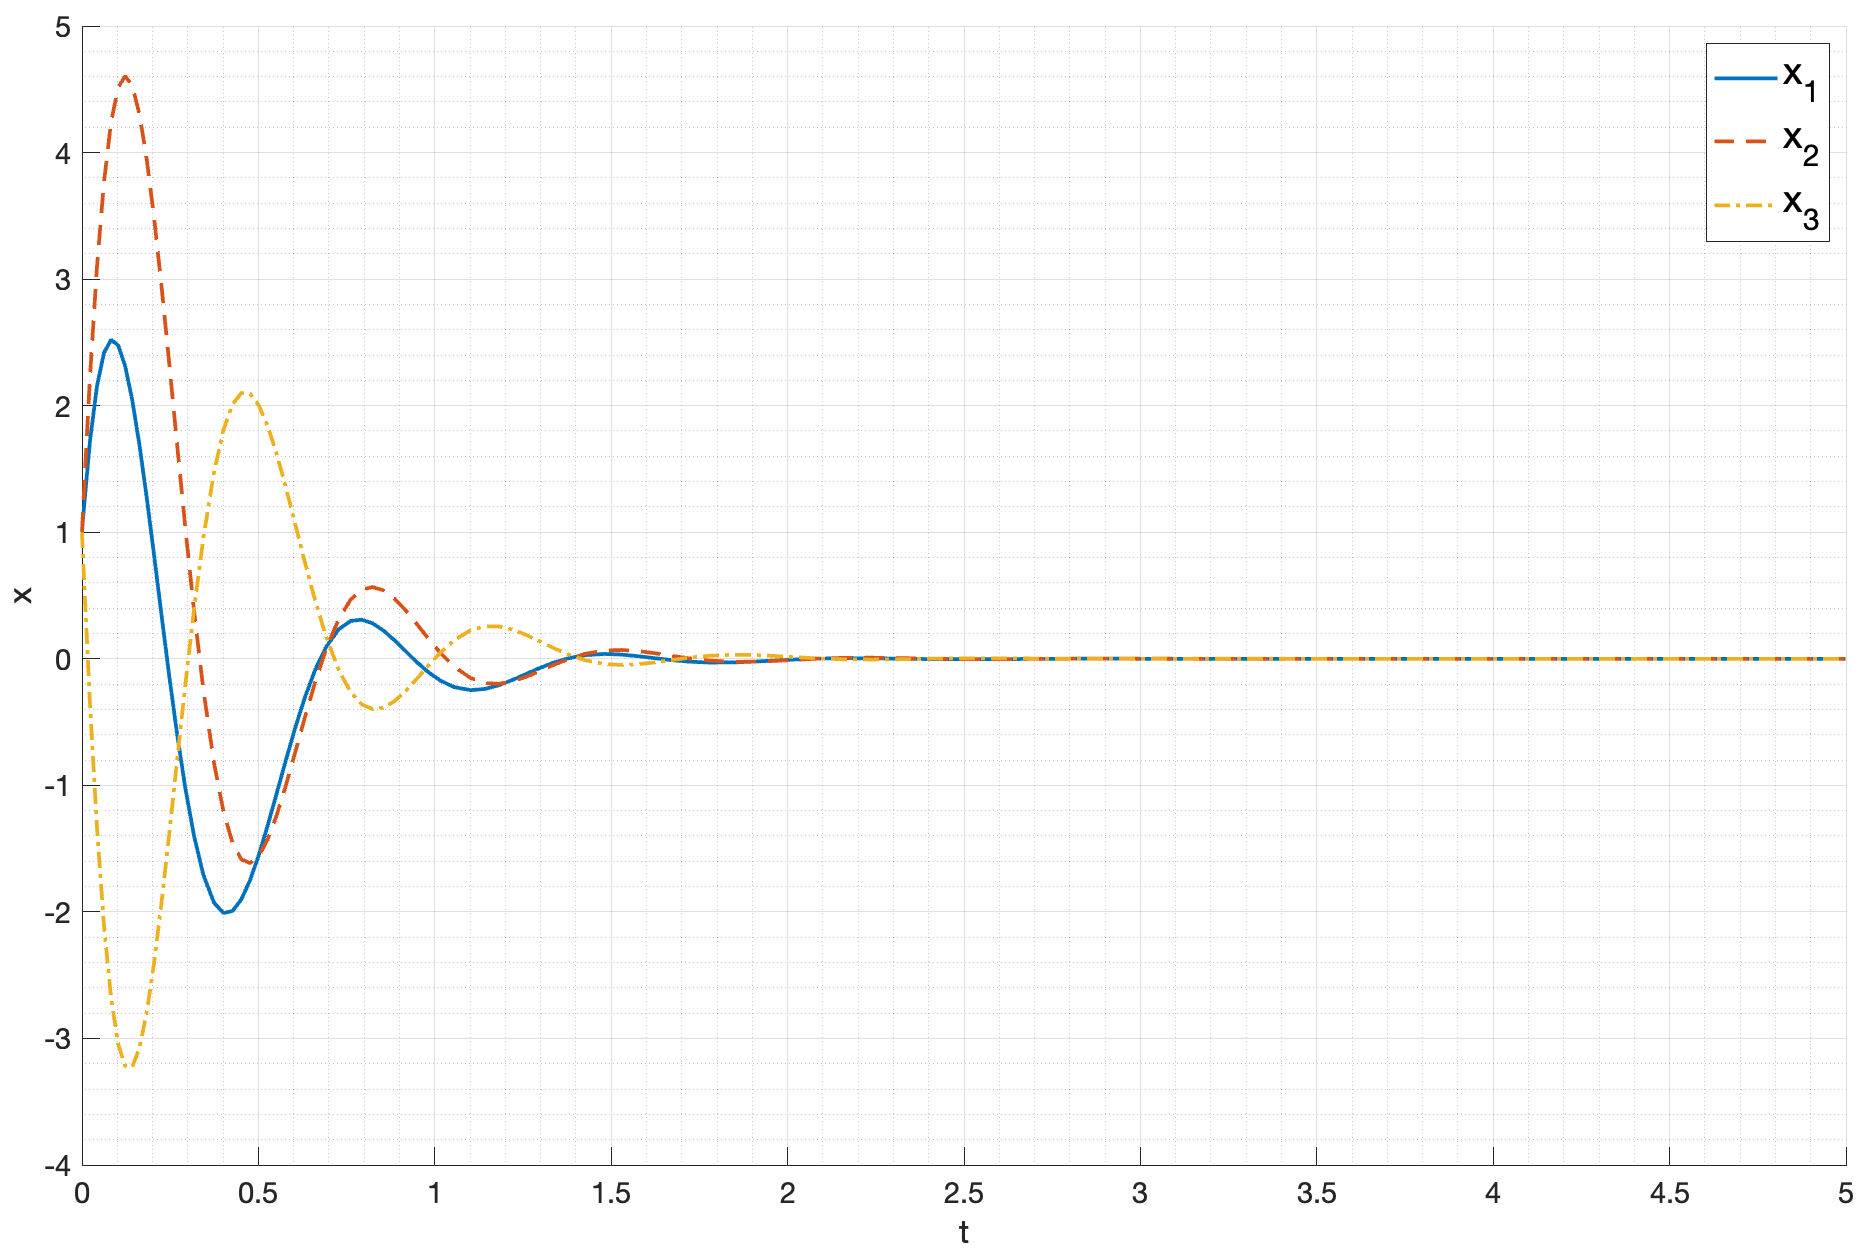
\includegraphics[width=\textwidth]{media/plots/task1_x_6.png}
    \caption{Состояние системы со спектром $\sigma_6$}
    \label{fig:task1_x_6}
\end{figure}

\subsubsection{Выводы}
В задании было показано, что для всех достижимых спектров эталонной системы можно найти модальный регулятор,
При этом, как и ожидалось на основании анализа спектра замкнутой системы, чем больше модуль
собственного числа, тем быстрее система приходит в устойчивое состояние, но при этом управление становится более интенсивным. 
Комплексная составляющая собственного числа вносит колебательный характер в систему. 